\documentclass{beamer}
\usepackage{animate}
\usepackage{tikz}
\usepackage{svg}
\usepackage{graphicx}
\usetheme{metropolis}
\begin{document}

\begin{frame}
  \begin{center}
    % Title
    {\LARGE Calibration with Machine Learning in Astronomy\par}
    \vspace{0.5cm}

    % First Author
    {\large Samuel Alan Kossoff Leeney\par}
    \vspace{0.5cm}

    % Institute
    {\normalsize Machine Learning for Astronomy 2024\par}

    % Date
    {\normalsize 14 November 2023\par}
    \vspace{1cm}

    % Co-authors
    {\footnotesize Co Authors: Harry Bevins, Will Handley, Eloy de Lera Acedo, Jiacong Zhu, Kaan Artuc, Daniel Molnar\par}
    \vfill

    % Image at the bottom
    
\includegraphics[width=0.9\textwidth]{affiliations.png}
  \end{center}
\end{frame}

\begin{frame}{\small{What is calibration in Astronomy?}}
\begin{figure}[h]
  \centering
  \includesvg[width=0.8\textwidth]{whatiscal.svg}
\end{figure}
\vfill
\tiny{sakl2@cam.ac.uk \hfill Sam Leeney \hfill \href{https://github.com/samleeney}{github.com/samleeney}}

\end{frame}


\begin{frame}{\small{How to calibrate?}}
\begin{figure}[h]
  \centering
  \includesvg[width=0.8\textwidth]{howtocal.svg}
\end{figure}
\vspace{0.7cm}
\tiny{sakl2@cam.ac.uk \hfill Sam Leeney \hfill \href{https://github.com/samleeney}{github.com/samleeney}}

\end{frame}


\begin{frame}{\small{Why is machine learning helpful?}}
\begin{figure}[h]
  \centering
  \includesvg[width=0.7\textwidth]{mlcal.svg}
\end{figure}
\vfill
\tiny{sakl2@cam.ac.uk \hfill Sam Leeney \hfill \href{https://github.com/samleeney}{github.com/samleeney}}
\end{frame}

\begin{frame}{\small{Machine learning for radiometer calibration in global 21cm cosmology}}
  \begin{figure}
    \centering
    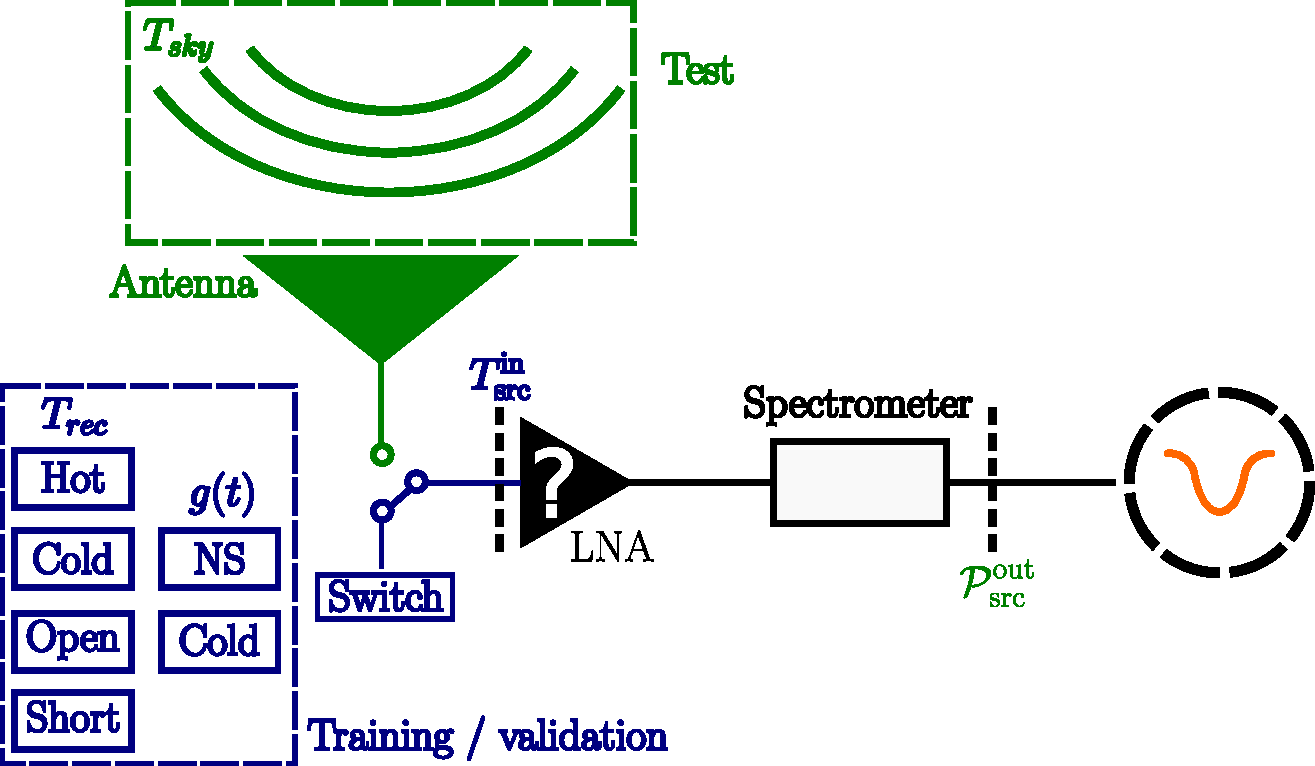
\includegraphics[width=1.05\textwidth]{instrument.pdf}
  \end{figure}
\vfill
\tiny{sakl2@cam.ac.uk \hfill Sam Leeney \hfill \href{https://github.com/samleeney}{github.com/samleeney}}
\end{frame}

\begin{frame}{\small{Machine learning for radiometer calibration in global 21cm cosmology}}
  \begin{figure}
    \centering
    \includesvg[width=0.9\textwidth]{nn.svg}
  \end{figure}
\vfill
\tiny{sakl2@cam.ac.uk \hfill Sam Leeney \hfill \href{https://github.com/samleeney}{github.com/samleeney}}
\end{frame}

\begin{frame}{\small{Machine learning for radiometer calibration in global 21cm cosmology}}
  \begin{figure}
    \centering
    \includesvg[width=1\textwidth]{results.svg}
  \end{figure}

  \begin{figure}
    \centering
    \includesvg[width=0.3\textwidth]{nn.svg}
  \end{figure}
\vfill
\tiny{sakl2@cam.ac.uk \hfill Sam Leeney \hfill \href{https://github.com/samleeney}{github.com/samleeney}}
\end{frame}

\begin{frame}{\small{Thank you!}}
  \begin{figure}
    \centering
    
\includegraphics[width=0.55\textwidth]{qr.png}
  \end{figure}
\end{frame}

\end{document}
